\chapter{Lecture 17}
\lhead{February 23, 2015}
\chead{21-366 Lambda Calculus Lecture 17}

\section{Reduction of Terms with Potential}
Recal that a potential is a sequence of nonnegative integers $n_1,n_2,\ldots,n_k$ such that $n_{i+1} = n_i \pm 1$. We now have three kinds of reductions we can perform:

\begin{eqnarray*}
  &\hbox{\hspace{.27in}\uline{Beta:} }& (1)\ \ ((\l x^{n,} X^{\alpha,n})^{n+1}Y^{\beta,n})^{n,\gamma} \rightarrow_\beta [Y^{\beta,n}/x^{n,}]X^{\alpha,n,\gamma}\\
  &\hbox{\uline{Potential:} }& (2)\ \ (U^{\alpha,n+2,n+1} V^{\beta,n})^{n,\gamma} \rightarrow (U^{\alpha,n+2} V^{\beta,n,n+1})^{n+1,n,\gamma}\\
  && (3)\ \ (U^{\alpha, n+1, n+2} V^{\beta,n+1})^{n+1, \gamma} \rightarrow (U^{\alpha, n+1} V^{\beta,n+1,n})^{n,n+1,\gamma}
\end{eqnarray*}
The above potential reductions are oftentimes referred to as ``rotations.''\\

Recall that we introduced potentials as a generalization of the idea of colored reductions. This raises a question: what corresponds to the case of colored redexes? We define every variable $x$ to have a potential of zero: $x^0$. Every instance of lambda abstraction gives us then $(\l x^0X^0)^{1,0}$. Our reductions stall, as this gives us $U^{0,1}V^2$.\\

If we assign a variable a potential of $1$, then our reductions do not stall. So this corresponds to a colored reduction. We have $U^1,V^1$.

\subsection{Weak Diamond with Potential Reduction}
We now consider a case where we have two terms $U$ and $V$ which both can be reduced using \textit{either} beta reduction or potential reduction from some third term $X$. The weak diamond property also holds in this case.
\begin{center}
  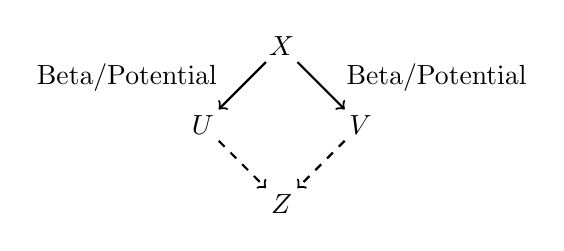
\begin{tikzpicture}
    \draw (0,0) node {$X$};
    \draw (-1,-1) node {$U$};
    \draw (1,-1) node {$V$};
    \draw (0,-2) node {$Z$};

    \draw[thick,->] (-.2,-.2) -- (-.8,-.8);
    \draw[thick,->] (.2,-.2) -- (.8,-.8);
    \draw[thick,dashed,->] (-.8,-1.2) -- (-.2,-1.8);
    \draw[thick,dashed,->] (.8,-1.2) -- (.2,-1.8);

    \draw (-.7,-.4) node[anchor=east] {Beta/Potential};
    \draw (.7,-.4) node[anchor=west] {Beta/Potential};
  \end{tikzpicture}
\end{center}

\textbf{Proof:} Consider $\Delta_1$ and $\Delta_2$ as $\beta$ redexes. There are four possible cases:
% The usual weak diamond picture with \Delta_1 and \Delta_2 as redexes
\begin{center}
  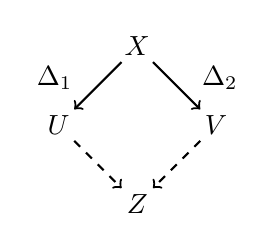
\begin{tikzpicture}
    \draw (0,0) node {$X$};
    \draw (-1,-1) node {$U$};
    \draw (1,-1) node {$V$};
    \draw (0,-2) node {$Z$};

    \draw[thick,->] (-.2,-.2) -- (-.8,-.8);
    \draw[thick,->] (.2,-.2) -- (.8,-.8);
    \draw[thick,dashed,->] (-.8,-1.2) -- (-.2,-1.8);
    \draw[thick,dashed,->] (.8,-1.2) -- (.2,-1.8);

    \draw (-.7,-.4) node[anchor=east] {$\Delta_1$};
    \draw (.7,-.4) node[anchor=west] {$\Delta_2$};
  \end{tikzpicture}
\end{center}
\begin{enumerate}[(1)]
  \item $\Delta_1$ and $\Delta_2$ are disjoint. This case is equivalent to the one without potentials.
  \item $\Delta_1$ is contained in $\Delta_2$
  \begin{enumerate}[(a)]
    \item $\Delta_1$ is contained in argument
    \item $\Delta_1$ is contained in abstraction terms
  \end{enumerate}
  \item Rotation/Rotation with $\Delta_1 \subseteq \Delta_2$. The diagram can be completed as in the case without potential.
  \item Rotation/Beta. There can be no conflict between a rotation and a beta reduction.
\end{enumerate}

\textbf{Definition:} We say that $X^{\alpha}$ is strongly normalizable SN if every reduction sequence terminates.

\section{Perpetual Strategy}
We define a \uline{principle redex} $\Delta$ such that if $X = X_0 \rightarrow X_1 \rightarrow X_2 \rightarrow \ldots \rightarrow X_n \rightarrow \infty$ sequence, then there is one with $\Delta$ as the first redex.\\

The principle redex of a term $X$ is
\begin{enumerate}[(1)]
  \item $X = (\l y^{n,}Y^{\beta,n})^{n+1,\alpha}$, then the principle redex is $Y^{\beta,n}$.
  \item $X = ((x^{\alpha,n+1}X_1^{\beta,n,})^{n_1}X_2^{\beta_2,N_1-1})\ldots X_n^{\boxed{\hphantom{lol}}}$, then
    \begin{enumerate}[(a)]
      \item The first $i$ such that $X_i$ has a principle redex.
      \item Else the principle redex is $x^{\alpha,n_+1}X_1^{\beta,n}$ if (1) or (2) apply
    \end{enumerate}
\end{enumerate}